
%(BEGIN_QUESTION)
% Copyright 2014, Tony R. Kuphaldt, released under the Creative Commons Attribution License (v 1.0)
% This means you may do almost anything with this work of mine, so long as you give me proper credit

A {\bf resistive tape} level sensor is a two-wire element immersed in a liquid, which changes resistance as liquid level increases.  The principle is the same as placing your rubber-boot-covered foot in a pool of water: the deeper your foot is submerged, the further up your foot and ankle you feel the water's pressure push the rubber boot against your skin.  A resistive tape stretches the entire height of the vessel, and contact is made between two resistive wires by the head pressure against the submerged length of the tape.  The greater the liquid level, the further the length that the two wires are in contact with each other, resulting in less resistance overall.

Examine the following resistive tape level measurement system and calculate the following, assuming a maximum tape resistance of 10 k$\Omega$ (i.e. resistance with zero immersion), a minimum resistance of 2 k$\Omega$ (i.e. resistance with total immersion), a linear relationship between tape immersion and tape resistance, and a total tape length of 15 feet:

$$\includegraphics[width=15.5cm]{i00855x01.eps}$$

Tape resistance ($R_{tape}$) = \underbar{\hskip 50pt}

\vskip 10pt

Immersion depth = \underbar{\hskip 50pt} 

\vfil 

\underbar{file i00855}
\eject
%(END_QUESTION)





%(BEGIN_ANSWER)

This is a graded question -- no answers or hints given!

%(END_ANSWER)





%(BEGIN_NOTES)

First, we need to determine the resistance of the tape.  Here, it is helpful to sketch an equivalent circuit:

$$\includegraphics[width=15.5cm]{i00855x02.eps}$$

If we know the tape drops 1.07 volts, then the 6.7 k$\Omega$ resistor must drop the remainder to make 3.5 volts (source voltage):

$$V_{6.7k} = 3.5 \hbox{ V} - 1.07 \hbox{ V} = 2.43 \hbox{ V}$$

This allows us to calculate total circuit current, since all current must flow through the 6.7 k$\Omega$ resistor:

$$I = {V \over R} = {2.43 \hbox{ V} \over 6700 \> \Omega} = 0.363 \hbox{ mA}$$

This 0.363 milliamp current splits when it reaches the parallel branches formed by the resistive tape and the 8.1 k$\Omega$ resistor.  We may calculate how much of this 0.363 milliamp current goes through the tape by calculating the 8.1 k$\Omega$ resistor's current and subtracting that amount of current from the 0.363 milliamp total (using Kirchhoff's Current Law).  First, calculating the 8.1 k$\Omega$ resistor current:

$$I = {V \over R} = {1.07 \hbox{ V} \over 8100 \> \Omega} = 0.132 \hbox{ mA}$$

Applying KCL to calculate tape current:

$$I_{tape} = 0.363 \hbox{ mA} - 0.132 \hbox{ mA} = 0.231 \hbox{ mA}$$

Now that we know how much current is passing through the resistive tape (0.231 mA), we may take the given voltage drop across the tape (1.07 volts) and calculate resistance using Ohm's Law:

$$R = {V \over I} = {1.07 \hbox{ V} \over 0.231 \hbox{ mA}} = 4640.3 \> \Omega$$

\vskip 10pt

\filbreak

Calculating immersion depth is an exercise in linear functions.  We know that the tape exhibits 10 k$\Omega$ of resistance when dry (0 feet immersion depth) and 2 k$\Omega$ resistance when fully immersed (15 feet immersion depth).  All we need to do is form a linear function relating immersion depth to resistance and then plug in our known resistance value of 4.6403 k$\Omega$ to solve for the depth of immersion in the given scenario:

$$\includegraphics[width=15.5cm]{i00855x03.eps}$$

Recall the standard slope-intercept formula for a linear function:

$$y = mx + b$$

\vskip 10pt

Calculating the slope ($m$) for this function:

$$m = \hbox{slope} = {\hbox{rise} \over \hbox{run}} = {2 - 10 \over 0 - 15} = - {8 \over 15}$$

\vskip 10pt

Plugging this slope into the $y = mx + b$ formula:

$$y = -{8 \over 15}x + b$$

\vskip 10pt

Solving for the y-intercept ($b$) value by plugging in any coordinate $x$ and $y$ values (in this case, 0 for $x$ and 10 for $y$):

$$10 = -\left({8 \over 15} \right) 0 + b$$

$$b = 10$$

\vskip 10pt

Writing the final $y = mx + b$ formula for this linear function:

$$y = -{8 \over 15}x + 10$$

\vskip 10pt

\filbreak

Now that we have a working formula describing this tape's resistance as a function of immersion depth, we may plug in the known resistance ($y$) and solve for immersion ($x$).  Note that since we developed our $y = mx + b$ function assuming resistance ($y$) in {\it kilo}-ohms rather than ohms, we must express our known tape resistance value as 4.6403 (kilo-ohms) rather than 4640.3 (ohms):

$$4.6403 = -{8 \over 15}x + 10$$

$$-5.3587 = -{8 \over 15}x$$

$$x = 10.049$$

Therefore, this tape is immersed in 10.049 feet of liquid.







%INDEX% Measurement, level: hydrostatic pressure

%(END_NOTES)

